\documentclass{article}

%\usepackage[landscape, centering, showcrop=true]{geometry} %
\usepackage[
%layoutheight=297mm,layoutwidth=450mm,  %420+thickness--here 30mm; estimate n*0.1/2 with 80g papers
%layoutvoffset=25mm,layouthoffset=30mm,
%paperheight=347mm,paperwidth=510mm,
paperheight=320mm,paperwidth=450mm,
margin=30mm,showcrop=false]{geometry}
%\usepackage[pdflatex,cam,center,a3,height=35cm,width=47cm]{crop} %

\usepackage[utf8]{inputenc}
%\usepackage[T1]{fontenc}

%%% FONT PACKAGES
%\usepackage[scaled=0.85]{beramono} % inconsolata or beramono ???
%\usepackage{fouriernc} % serif: new century schoolbook
\usepackage{avant}     % sans serif: Avant Garde
\usepackage{microtype} % Slightly tweak font spacing for aesthetics
%\usepackage{changepage}   % for the adjustwidth environment to make narrow paragraphs

\usepackage{sectsty} %change font on headings
\allsectionsfont{\sffamily}


\usepackage{tikz}
\usetikzlibrary{calc}

\newcommand{\YEAR}{2016}

\begin{document}

\newcommand{\LeftMarginBack}{1.0}
\newcommand{\RightMarginFront}{1.0}
\newcommand{\YPosFront}{-1.5}
\newcommand{\YPosBack}{0}

\thispagestyle{empty}
\renewcommand{\familydefault}{\sfdefault}
\renewcommand{\arraystretch}{1.5}
%\newgeometry{a3paper,landscape, centering}
%\makeatletter\CROP@center\makeatother

\begin{tikzpicture}[overlay,remember picture]%[overlay,remember picture]
    \fill[red,fill opacity=0.3] (current page.south west) rectangle (current page.north east);
    \node[text width=250mm, align=right] (intro) at ($(current page.north east)+(-14.5,-6.5)-(\RightMarginFront,\YPosFront)$) {
       \fontsize{28}{46}\sffamily\selectfont\textbf{Introduktion~~till} 
       };  
       
    \node[text width=250mm, align=right] (prog) at ($(current page.north east)+(-14.5,-8.5)-(\RightMarginFront,\YPosFront)$) {
       \fontsize{52}{46}\sffamily\selectfont\textbf{programmering} 
       };        

    \node[text width=250mm, align=right] (prog) at ($(current page.north east)+(-14.5,-28.8)-(\RightMarginFront,\YPosFront)$) {
       \fontsize{28}{46}\sffamily\selectfont{med~~Scala~~och~~Java} 
       };        
    
    \node[text width=250mm, align=right] (prog) at ($(current page.north east)+(-14.5,-30.0)-(\RightMarginFront,\YPosFront)$) {
       \fontsize{18}{46}\sffamily\selectfont\texttt{http://cs.lth.se/pgk} 
       };    

    %\node[text width=250mm, align=right] (prog) at ($(current page.north east)+(-14.5,-28.2)$) {
    %   \fontsize{18}{46}\sffamily\selectfont  2016
    %   }; 
   

    \node[above right] (picture) at ($(current page.north east)+(-16,-26.8)-(\RightMarginFront,\YPosFront)$) {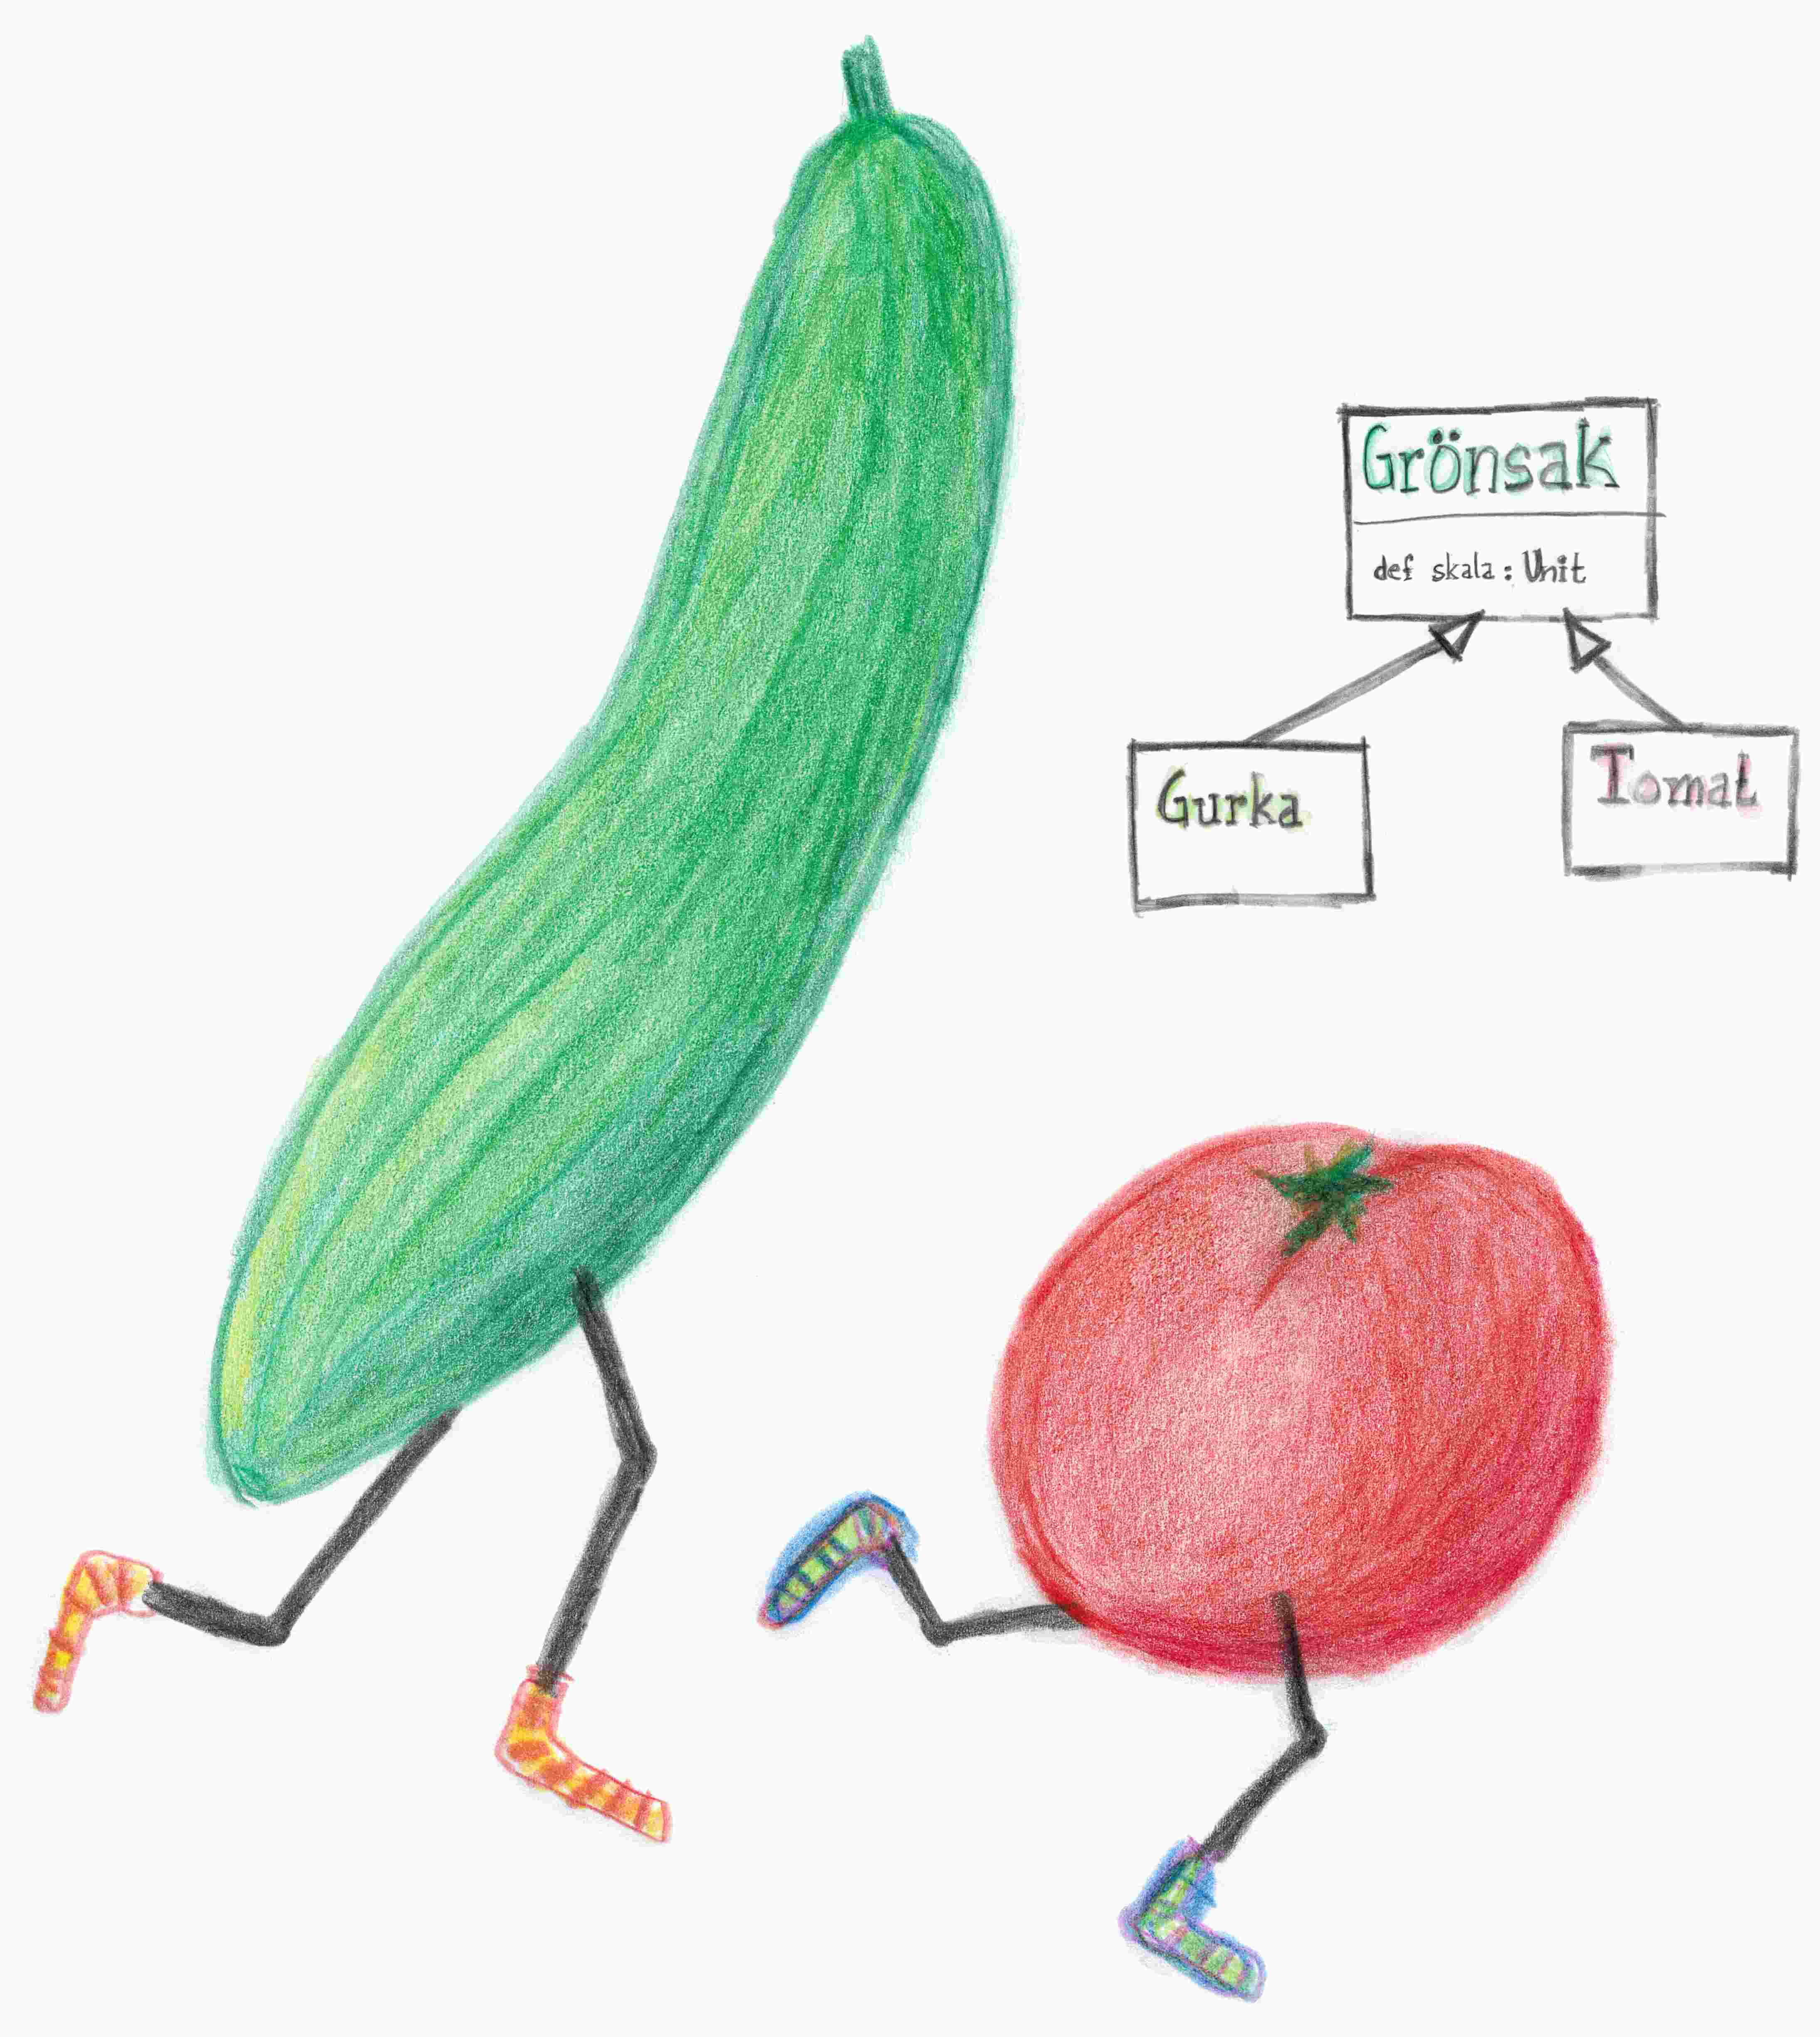
\includegraphics[width=140mm]{gurka.jpg}};
    
    
\node[above right] (logo) at ($(current page.west)+(19.0,-21.8)+(2.5,0.5)$) {
\includegraphics[scale=0.54]{logoLUeng}};

    
        
\node[anchor=north,rotate=-90, align=left] (back) at ($(current page.north)+(0.0,-11.8)+(0,-3.0)$) {
\fontsize{18}{20}\sffamily\selectfont\textbf{Introduktion till programmering med Scala och Java} \hspace{2.0cm}\texttt{http://cs.lth.se/pgk}};

\node[anchor=north] (back) at ($(current page.north)+(-0.4,-15.0)+(0,-4.3)$) {
\fontsize{16}{20}\sffamily\selectfont {\YEAR}};



\node[above right, scale=1.3] (modulplan) at ($(current page.west)+(\LeftMarginBack,-11.5)+(1.0,\YPosBack)$) {
\sffamily\begin{tabular}{l|l|l|l}
\textit{W} & \textit{Modul} & \textit{Övn} & \textit{Lab} \\ \hline \hline
W01 & Introduktion         & expressions & kojo            \\
W02 & Kodstrukturer        & programs    & --              \\
W03 & Funktioner, Objekt   & functions   & simplewindow    \\
W04 & Datastrukturer       & data        & textfiles       \\
W05 & Vektoralgoritmer     & vectors     & cardgame        \\
W06 & Klasser, Likhet      & classes     & shapes          \\
W07 & Arv, Gränssnitt      & traits      & turtlerace-team \\
KS  & KONTROLLSKRIVN.      & --          & --              \\
W08 & Mönster, Undantag    & matching    & chords-team     \\
W09 & Matriser             & matrices    & maze            \\
W10 & Sökning, Sortering   & sorting     & surveydata-team \\
W11 & Scala och Java       & scalajava   & scalajava-team  \\
W12 & Trådar, Web, Android & threads     & life            \\
W13 & Design               & Uppsamling  & Inl.Uppg.       \\
W14 & Tentaträning         & Extenta     & --              \\
T   & TENTAMEN             & --          & --              \\
\end{tabular}
 
};

\node[above right, text width=15cm,align=left] (collection-traits) at ($(current page.west)+(\LeftMarginBack,3.8)+(1.0,\YPosBack)$) {
\begin{minipage}{1.0\textwidth}\sffamily\large 
Detta kompendium är kurslitteratur i grundkursen i programmering på Datateknikprogrammet vid Lunds tekniska högskola.

\vspace{1em}
I kursen används språken Scala och Java för att illustrera grunderna i imperativ och objektorienterad programmering, samt elementär funktions-programmering.  

\vspace{1em}
En viktig framgångsfaktor vid studier i programmering är att du bejakar din egen upptäckarglädje och experimentlusta. Det är kul när du med nya kunskaper kan skapa fungerande program, men minst lika lärorikt är felsökning, buggrättande och misslyckade försök som, ibland efter hårt arbete, vänds till lyckade lösningar och bestående lärdomar.

\vspace{1em}
Läromaterialet fokuserar därför på lärande genom praktiskt programmeringsarbete och innehåller övningar och laborationer som är organiserade i moduler enligt en noga uttänkt progression, där dina kunskaper utvecklas steg för steg. Varje modul har ett tema enligt tabellen nedan. 



\vspace{1em}
Välkommen till datavetenskapens fascinerande värld!
\end{minipage}
};

\node[above right, scale=1.3] (modulplan) at ($(current page.west)+(\LeftMarginBack,-13.5)+(1.0,\YPosBack)$) {
\begin{minipage}{0.33\textwidth}
\sffamily Datavetenskap, LTH, Lunds universitet. Licens: CC-BY-SA. Upplaga \YEAR. \\ \texttt{http://cs.lth.se/pgk}
\end{minipage}
};


%\node[above right] (collection-traits) at ($(current page.west)+(4.0,-9.5)$) {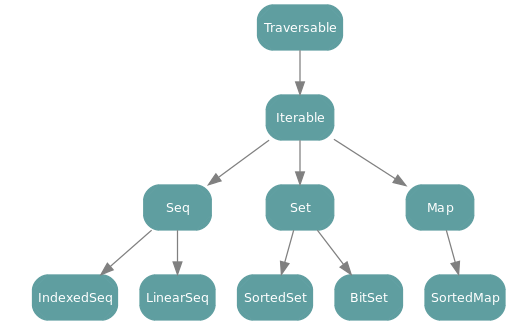
\includegraphics[scale=0.55]{../../img/collection/collection-traits}};

%
%
%\node[above right] (collection-traits) at ($(current page.west)+(1.0,7.5)$) {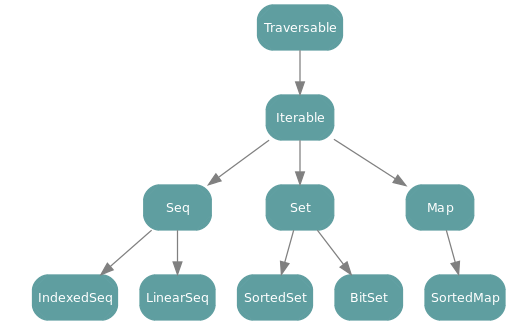
\includegraphics[scale=0.55]{../../img/collection/collection-traits}};
%
%\node[above right] (collection-traits-text) at ($(current page.west)+(1.0,12.5)$) {\texttt{\large scala.collection}};
%
%\node[above right] (collection-legend) at ($(current page.west)+(14.0,7.5)$) {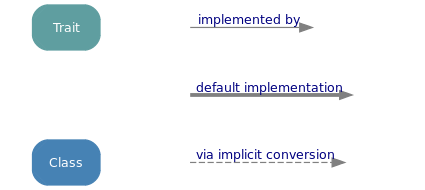
\includegraphics[scale=0.30]{../../img/collection/collection-legend}};
%
%\node[above right] (collection-immutable) at ($(current page.west)+(2,-3.4)$) {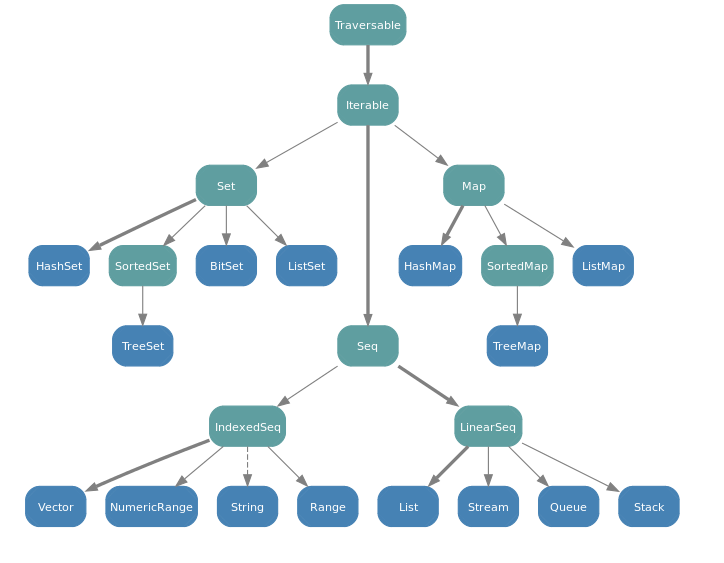
\includegraphics[scale=0.50]{../../img/collection/collection-immutable}};
%
%\node[above right] (collection-traits-text) at ($(current page.west)+(1.0,4.5)$) {\large\texttt{\large immutable}};
%
%\node[above right] (collection-mutable) at ($(current page.west)+(0,-15.2)$) {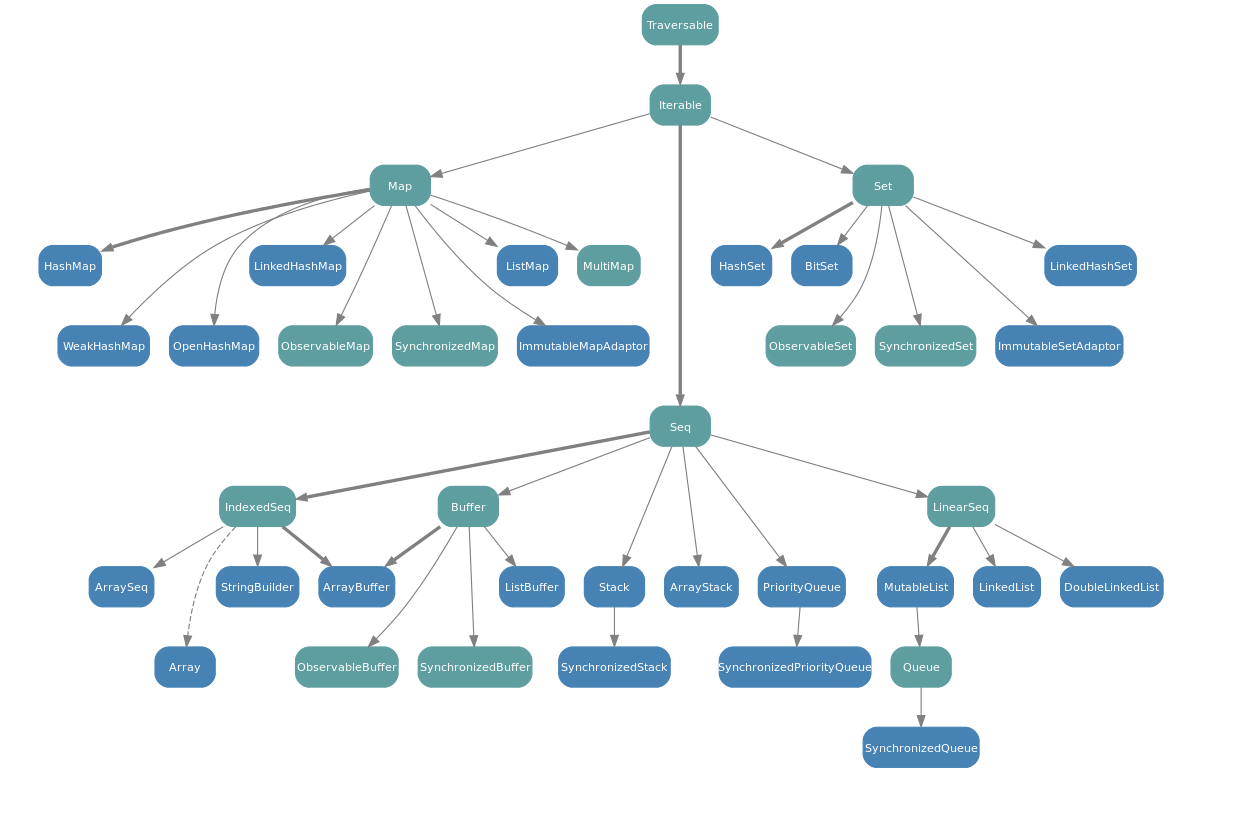
\includegraphics[scale=0.40]{../../img/collection/collection-mutable}};
%
%\node[above right] (collection-traits) at ($(current page.west)+(1.0,-5.5)$) {\texttt{\large mutable}};



% ../../img/collection/collection-immutable
\end{tikzpicture}
\end{document}